% =====================================================================================
% DRAFT for IEEE DG 2027 -- orientation draft, to be rewritten by the author.
% Every number of this study is taken from results/*.csv; the source is given in a
% % comment next to it (key names refer to results/paper_numbers.csv, built by
% src/paper_numbers.py). Tables are generated by src/paper_numbers.py.
% Markers: [CHECK] = not confirmed by results or sources; [REF NEEDED] = no verified reference.
% Scope of inference: significance statements only for h = 1 and h = 7; h = 28 is descriptive
% (see results/h28_inference.md).
% Build: tectonic main.tex   (from paper/)
% =====================================================================================
\documentclass[conference]{IEEEtran}
\usepackage[T1]{fontenc}
\usepackage{cite}
\usepackage{amsmath,amssymb}
\usepackage{graphicx}
\usepackage{booktabs}
\usepackage{xcolor}
\usepackage{url}
\graphicspath{{../figures/}}
\newcommand{\CHECK}[1][]{\textcolor{red}{\textbf{[CHECK#1]}}}
\newcommand{\REFNEEDED}[1]{\textcolor{red}{\textbf{[REF NEEDED: #1]}}}

\begin{document}

\title{Do Lagged Operational KPIs Improve Daily Revenue Forecasts? A Leakage-Safe Ablation on Online Retail Data}

\author{\IEEEauthorblockN{Amir Nurseit}
\IEEEauthorblockA{Applied Data Analytics\\
Astana IT University\\
Astana, Kazakhstan\\
a2n19a2n@gmail.com}
\and
\IEEEauthorblockN{Zhanar Beldeubayeva}
\IEEEauthorblockA{Astana IT University\\
Astana, Kazakhstan\\
zh.beldeubayeva@astanait.edu.kz}}

\maketitle

\begin{abstract}
Business KPIs such as orders, active customers and average order value (AOV) are mechanically linked to
revenue, which makes them attractive predictors but also an easy source of data leakage. We study whether
\emph{lagged} operational KPIs improve daily revenue forecasts when evaluated under a leakage-safe
protocol. Using the UCI Online Retail II transactions, we compare a model that uses only revenue history and
calendar information (Model~A) with one that adds lagged orders, active customers, AOV and cancellation rate
(Model~B), for Ridge, random forest and LightGBM, against seasonal naive, ETS and SARIMA baselines. Forecasts
are evaluated by expanding-window rolling origin over 305 target days % metrics.csv: n (test_days)
with MASE; significance is assessed with Diebold--Mariano tests with the Harvey--Leybourne--Newbold
correction at horizons of 1 and 7 days, while a 28-day horizon is reported descriptively. With squared-error
loss, all eight learned and statistical configurations significantly outperform the seasonal naive baseline % dm_tests.csv: n_sig_vs_sn_se_h1, n_sig_vs_sn_se_h7 (8, 8)
at 1 and 7 days; with absolute-error loss the six ML configurations still do, but ETS does not. % dm_tests.csv: n_sig_vs_sn_ae_h1 (7), n_sig_vs_sn_ae_h7 (6); p_holm_ae_ets_vs_sn_h1/h7
The best MASE is 0.752 (random forest, $h=1$). % metrics.csv: mase_rev_random_forest_A_h1
No statistically significant improvement from the lagged drivers was detected in any of 18 comparisons at 1 and 7 days, % dm_tests.csv: n_b_vs_a_h17_se, n_b_better_sig_h17_se, n_b_better_sig_h17_ae
with relative MASE changes between $-3.2\%$ and $+4.1\%$ across all three targets % metrics.csv: rel_b_vs_a_h17_min_pct, rel_b_vs_a_h17_max_pct
($-3.2\%$ to $+0.6\%$ for revenue), % metrics.csv: rel_b_vs_a_rev_h17_min_pct, rel_b_vs_a_rev_h17_max_pct
and a post hoc ablation by driver group found no significant difference either. % ablation_groups.csv: abl_n_sig_h1h7_*
A control experiment that adds the target day's own KPIs to the features reduces MASE to 0.16--0.24; % leakage_control.csv: leak_mase_min/max (all horizons, descriptive)
the MASE of the legitimate models is 3.4--4.8 times that of the leaky ones, although the added target-day % leakage_control.csv: leak_ratio_min/max (= MASE legal B / MASE leaky)
features are unavailable at the forecast origin.
\end{abstract}

\begin{IEEEkeywords}
KPI forecasting, data leakage, rolling-origin evaluation, Diebold--Mariano test, retail analytics, SHAP
\end{IEEEkeywords}

% =====================================================================================
\section{Introduction}
Revenue forecasts support inventory, staffing and budgeting decisions, and retail organizations increasingly
produce them with machine learning (ML) models trained on transaction data~\cite{fildes2022}. Transaction
data also yield operational KPIs: the number of orders, active customers, AOV and the cancellation rate.
Because revenue equals orders times AOV, these KPIs are natural candidate predictors. The same identity makes
them dangerous: if a same-period KPI enters the feature set, the model partly reconstructs the target instead
of forecasting it. Such leakage produces accuracy estimates that cannot be reproduced at forecast
time~\cite{kaufman2012leakage}, and evaluation pitfalls of this kind are common in applied forecasting
work~\cite{hewamalage2023}.

This paper asks a narrow question: \emph{when only information available at the forecast origin is used, do
lagged operational KPIs improve daily revenue forecasts?} We answer it with a controlled ablation on a
public dataset. Our contribution is methodological and deliberately modest:
\begin{itemize}
\item a leakage-safe forecasting protocol (expanding-window rolling origin, direct multi-horizon strategy,
train-only preprocessing, automated leakage tests) with the main settings fixed in a configuration
file before the backtest and later additions marked as post hoc;
\item a controlled ablation of feature groups (revenue history and calendar vs.\ the same plus lagged driver
KPIs) with Diebold--Mariano tests corrected for small samples and multiple comparisons;
\item a leakage control experiment that quantifies how much same-period KPIs overstate accuracy.
\end{itemize}
We address three research questions. RQ1: are ML models (Ridge, random forest, LightGBM) significantly more
accurate than the seasonal naive and ETS baselines for daily revenue at 1 and 7 days (SARIMA is compared with
the seasonal naive baseline only)? RQ2: does adding lagged driver
KPIs (Model~B) significantly improve on revenue history and calendar alone (Model~A) at 1 and 7 days? RQ3: how
do accuracy and feature-group attributions change from 1 to 28 days (descriptively)?

% =====================================================================================
\section{Related Work}
Large comparisons of statistical and ML forecasting methods showed that ML methods do not automatically
outperform simple statistical baselines~\cite{makridakis2018}, while on tabular data tree ensembles remain
strong compared with deep networks~\cite{grinsztajn2022}. Retail forecasting has a long research tradition
that stresses hierarchies, promotions and calendar effects~\cite{fildes2022}. The one-year predecessor of our
dataset, Online Retail (December~2010 to December~2011), was introduced with a study of RFM-based customer % source: UCI API metadata, dataset id 352 (intro_paper = chen2012rfm; 01/12/2010-09/12/2011); paper itself not read
segmentation~\cite{chen2012rfm}, not with a time-series forecasting task. Arantes et al.~\cite{arantes2025}
examined the trade-off between predictive accuracy and interpretability in daily retail sales forecasting
using Rossmann store data.
% source: full text of arantes2025 read 2026-11-03 (abstract; Sec. 3: daily sales of Rossmann stores, XGBoost vs. linear regression, hybrid LR XGBoost)

Evaluation methodology is central to our design. Rolling-origin out-of-sample evaluation is the standard way
to assess forecasts~\cite{tashman2000}; cross-validation for autoregressive models is valid only under
conditions discussed in~\cite{bergmeir2018}; and \cite{hewamalage2023} list frequent pitfalls, including
leakage and inappropriate error measures. We use the mean absolute scaled error (MASE), which is defined
for series with zeros~\cite{hyndman2006}, and compare forecasts with the Diebold--Mariano (DM)
test~\cite{diebold1995} with the small-sample correction of Harvey, Leybourne and Newbold
(HLN)~\cite{harvey1997}. For explanation we use SHAP values~\cite{lundberg2017shap}.

A related study is a recent preprint by Kim, McCarthy and Lee~\cite{kim2026drivers}, who forecast revenue
jointly with its customer-base primitives (acquisition, repeat purchasing, spend per order) using weekly
panels of 966 companies. Their multi-task model reduced total-sales error by 2.65\% relative to a Transformer
forecasting total sales directly, but the paired difference was not statistically significant
($p=.222$). % numbers from the arXiv abstract of kim2026drivers, not from our results
Our study differs in scope: a single retailer at daily frequency, classical and tree-based models, and an
explicit ablation of lagged driver KPIs under a leakage-safe protocol. As a preprint, \cite{kim2026drivers}
has not yet been peer reviewed.

% =====================================================================================
\section{Data and Protocol}
\subsection{Data and cleaning}
We use UCI Online Retail II~\cite{chen2012dataset}: 1,067,371 transaction lines % data_profile.csv: raw_rows
of a UK-based online retailer from 1~December~2009 to 9~December~2011. The two Excel sheets overlap from 1
to 9~December~2010 with 22,523 identical lines, % cleaning_log.csv: R1 (overlap_rows)
which we keep only once. We further remove exact duplicates, bad-debt adjustments, lines with non-positive
price, accounting, fee and test codes, postage lines, and two erroneous orders of more than 50{,}000 units
that were cancelled within minutes. 1,021,346 lines remain. % cleaning_log.csv: clean_rows
Cancellations (17,914 lines) % cleaning_log.csv: cancel_rows
are kept and used for the cancellation rate; lines without a customer identifier are kept for revenue and
orders. The last day (9~December~2011) ends at 12:50 and is excluded. Every rule, with the number of affected
lines and the revenue involved, is logged.

\subsection{KPIs and calendar}
Daily KPIs are computed on a full calendar of 738 days, of which 603 are trading days. % daily_kpis_summary.csv: calendar_days, trading_days
Revenue is the gross merchandise revenue of non-cancelled lines; orders and active customers are distinct
invoices and customer identifiers; AOV is revenue per order; the cancellation rate is the share of cancelled
invoices. The retailer does not trade on Saturdays (one Saturday with sales in the whole period), % daily_kpis_summary.csv: sat_trading_days
on UK bank holidays and around Christmas. On the calendar series the autocorrelation at lag~7 is 0.64, % eda_seasonality.csv: acf7
and the in-sample MAE of the seasonal naive forecast is 10,599 with period~7, against 16,850 with period~6 % eda_seasonality.csv: snaive_mae_m7, snaive_mae_m6
and 15,830 for the one-day naive forecast. % eda_seasonality.csv: naive1_mae
We therefore keep the 7-day calendar with zero revenue on non-trading days and use a seasonal period of
$m=7$.

\subsection{Forecasting protocol}
The test period runs from 7~February to 8~December~2011 (305 target days per horizon). % metrics.csv: test_days
It starts on the first Monday for which no forecast origin and no seasonal reference falls into the
Christmas closure. For a target day $T$ and horizon $h\in\{1,7,28\}$ the forecast origin is $T-h$ and the
training set contains only targets observed up to $T-h$ (expanding window, direct strategy). All models are
evaluated on exactly the same target days. Statistical models are re-estimated at every origin; ML models
are re-estimated every seven days on all data up to the origin, while their lag features are always current.
Hyperparameters are fixed in advance (no tuning on the test period); the Ridge penalty is selected by
generalized cross-validation on the training window only. All settings were fixed in a configuration file
before the backtest was run; the file was committed together with the first results, so the version history
does not independently document this order. Analyses added after the main results (the no-Saturday tests,
the feature-group ablation and the Bartlett sensitivity check) are marked as post hoc and logged in the
configuration file.

\subsection{Features}
Model~A uses revenue lags $h,\dots,h+6$ and the first four weekly lags not smaller than $h$, rolling means and
standard deviations over 7 and 28 days of the series shifted by $h$, and calendar indicators (day of week,
month, UK bank holiday, Christmas period), which are known in advance. Model~B adds lags $h,\dots,h+6$ and a
7-day rolling mean (shifted by $h$) of orders, active customers, AOV and cancellation rate.

Leakage is tested automatically. Each lag must be at least $h$; same-period KPIs are forbidden; and a
perturbation test overwrites all KPI values after $T-h$ with random noise and requires the features at $T$
to be unchanged. These checks run in the unit tests and at every step of the backtest; a deliberately leaky
feature set fails all three.

\subsection{Models, metrics and tests}
Baselines are the seasonal naive forecast ($m=7$), additive ETS~\cite{hyndman2002} and
SARIMA$(1,0,1)(0,1,1)_7$~\cite{box2015}. ML models are Ridge
regression~\cite{hoerl1970} with standardization, random forest~\cite{breiman2001} (300 trees, minimum leaf
size 3) and LightGBM~\cite{ke2017lightgbm} (300 trees, learning rate 0.05, 15 leaves).

The primary metric is MASE~\cite{hyndman2006}. Each error is scaled by the in-sample MAE of the seasonal
naive forecast (lag 7) on the data available at its own origin; MASE is the mean of these scaled errors. We
also report MAE, RMSE and WAPE. MAPE is not used because of zero-revenue days. Forecast accuracy is compared
with the DM test~\cite{diebold1995} with the HLN correction~\cite{harvey1997}, using autocovariances up to lag
$h-1$ with equal weights, squared-error loss (absolute-error loss as robustness) and Holm
adjustment~\cite{holm1979}. A Holm family is one target $\times$ horizon $\times$ comparison type $\times$ loss
function; for Model~B vs.\ Model~A a family therefore holds 3 tests, one per ML model. % dm_tests.csv: holm_family_size_b_vs_a; code: src/backtest.py run_dm groupby(target, h, family, loss)
Each model is compared with the seasonal naive forecast, each ML configuration with ETS, and Model~B with
Model~A; ML models are not tested against SARIMA. Squared error is the protocol loss; because MASE is an
absolute-error measure, absolute-error results are reported alongside. Significance is interpreted for $h=1$
and $h=7$ only; $p$-values for $h=28$ are computed and stored with the results but not interpreted, because
the variance estimator is unreliable at this horizon (Section~\ref{sec:limits}). As a post hoc sensitivity
check, all tests are repeated with Bartlett weights $1-k/h$.

% =====================================================================================
\section{Experiments}
The backtest covers three targets (revenue, orders, active customers), three horizons, six models and two
feature sets, plus the leakage control. This paper focuses on revenue; orders and active customers are
reported for the B-vs-A comparison only. The leakage control repeats Model~B for Ridge and LightGBM and adds
the values of orders, active customers, AOV, cancellation rate and quantity sold on the target day itself. % src/features.py: LEAKY_SAME_DAY (*_lag0 features)
Feature attributions are computed with TreeSHAP for every out-of-sample LightGBM forecast and aggregated by feature group; group
permutation importance is computed as a cross-check. The code, experiment configurations, and result files are
available at \url{https://github.com/A2N19/retail-kpi-forecasting}. The full backtest
runs in under 7 minutes on a laptop CPU. % results/run_all_log.csv: backtest 410.2 s (fresh environment)

% =====================================================================================
\section{Results}
\subsection{RQ1: models vs.\ baselines}
Table~\ref{tab:mase} reports MASE for daily revenue. With squared-error loss, all eight configurations (ETS,
SARIMA and the six ML configurations) are significantly more accurate than the seasonal naive forecast at % dm_tests.csv: n_sig_vs_sn_se_h1, n_sig_vs_sn_se_h7 (8, 8)
$h=1$ and $h=7$ (Holm-adjusted DM-HLN $p<0.05$), also with Bartlett weights. % dm_tests_bartlett.csv: n_sig_vs_sn_bartlett_h1, n_sig_vs_sn_bartlett_h7 (8, 8; SE)
With absolute-error loss, all six ML configurations remain significant, but ETS does not ($p=0.058$ at $h=1$, % dm_tests.csv: n_sig_vs_sn_ae_h1 (7), p_holm_ae_ets_vs_sn_h1
$p=0.149$ at $h=7$) and neither does SARIMA at $h=7$ ($p=0.053$). % dm_tests.csv: n_sig_vs_sn_ae_h7 (6), p_holm_ae_ets_vs_sn_h7, p_holm_ae_sarima_vs_sn_h7
Random forest has the lowest MASE at both horizons: with Model~A at $h=1$ (0.752) and with Model~B at $h=7$ % metrics.csv: mase_rev_random_forest_A_h1; best_models.csv
(0.756, ahead of Model~A by less than 0.001), % metrics.csv: mase_rev_random_forest_B_h7 (0.7557) vs mase_rev_random_forest_A_h7 (0.7561); best_models.csv
corresponding to a WAPE of about 0.28. % metrics.csv: wape_rev_rfA_h1, wape_rev_rfA_h7
The comparison with ETS depends on the loss. With absolute error, 4 of 6 ML configurations (Ridge and random
forest, both feature sets) are significantly more accurate than ETS at $h=1$, and 6 of 6 at $h=7$
(Holm-adjusted).
% dm_tests.csv: n_sig_vs_ets_ae_h1 (4), n_sig_vs_ets_ae_h7 (6)
With squared error, only random forest with Model~A at $h=7$ is significant, and only with Bartlett weights;
% dm_tests_bartlett.csv: n_sig_vs_ets_bartlett_h7 (SE, 1)
with the protocol variance no configuration is significant after the Holm adjustment, although 4 of 6 at
$h=1$ and 5 of 6 at $h=7$ have unadjusted $p<0.05$.
% dm_tests.csv: n_sig_vs_ets_se_h1, n_sig_vs_ets_se_h7 (0, 0); n_rawsig_vs_ets_h1, n_rawsig_vs_ets_h7 (SE)
Across all tests at $h=1$ and $h=7$, 7 of 204 decisions differ between the two variance estimators. % dm_tests_bartlett.csv: n_dm_decisions_changed_bartlett_h17, n_dm_tests_h17
ML models were not tested against SARIMA; the MASE values in Table~\ref{tab:mase} are descriptive for this
comparison. At $h=28$, reported descriptively, ETS and SARIMA have MASE 0.920 and 0.960 and all ML % metrics.csv: mase_rev_ets_-_h28, mase_rev_sarima_-_h28; tab_mase_revenue.tex
configurations stay below 0.83; the corresponding $p$-values are not interpreted (Section~\ref{sec:limits}).

% Generated by src/paper_numbers.py from results/metrics.csv (target=revenue, subset=all_days)
\begin{table}[t]
\centering
\caption{Test-period MASE for daily revenue (305 target days per horizon). Set A: revenue history and calendar; set B: A plus lagged driver KPIs. Lower is better; best per horizon in bold (determined before rounding). Significance tests: see text (ML vs.\ SARIMA not tested); $h=28$ is descriptive ($p$-values not interpreted, Section~\ref{sec:limits}).}
\label{tab:mase}
\begin{tabular}{llccc}
\toprule
Model & Set & $h=1$ & $h=7$ & $h=28$ \\
\midrule
Seasonal naive & -- & 0.981 & 0.980 & 1.065 \\
ETS & -- & 0.872 & 0.915 & 0.920 \\
SARIMA & -- & 0.838 & 0.861 & 0.960 \\
Ridge & A & 0.796 & 0.799 & 0.818 \\
Ridge & B & 0.792 & 0.804 & 0.826 \\
Random forest & A & \textbf{0.752} & 0.756 & \textbf{0.758} \\
Random forest & B & 0.755 & \textbf{0.756} & 0.769 \\
LightGBM & A & 0.849 & 0.799 & 0.787 \\
LightGBM & B & 0.833 & 0.773 & 0.785 \\
\bottomrule
\end{tabular}
\end{table}


\subsection{RQ2: lagged driver KPIs}
Table~\ref{tab:bva} and Fig.~\ref{fig:bva} compare Model~B with Model~A at $h=1$ and $h=7$. For revenue the
relative change in MASE lies between $-3.2\%$ and $+0.6\%$. % metrics.csv: rel_b_vs_a_rev_h17_min_pct, rel_b_vs_a_rev_h17_max_pct
No significant difference was detected in any of the 18 comparisons across the three targets, two horizons and % dm_tests.csv: n_b_vs_a_h17_se, n_b_better_sig_h17_*, n_b_worse_sig_h17_*
three models, under either loss, with either variance estimator or without Saturdays. % dm_tests_bartlett.csv: n_b_sig_any_bartlett_h17; dm_tests_no_saturdays.csv: n_b_sig_any_nosat_h17_*
This is a null result: with 305 test days per horizon, our design did not detect a gain from lagged drivers;
it does not show that such a gain cannot exist.

% Generated by src/paper_numbers.py from results/metrics.csv and results/dm_tests.csv
\begin{table}[t]
\centering
\caption{Model B (with lagged driver KPIs) vs Model A for daily revenue. $\Delta$MASE $=$ (B$-$A)/A; $p$: DM-HLN, Holm-adjusted within each target $\times$ horizon $\times$ comparison type $\times$ loss family (3 tests: one per model); SE and AE loss.}
\label{tab:bva}
\begin{tabular}{llrcc}
\toprule
$h$ & Model & $\Delta$MASE, \% & $p_{\mathrm{SE}}$ & $p_{\mathrm{AE}}$ \\
\midrule
1 & Ridge & -0.5 & 1.000 & 1.000 \\
1 & Random forest & +0.3 & 1.000 & 1.000 \\
1 & LightGBM & -1.9 & 1.000 & 1.000 \\
\addlinespace
7 & Ridge & +0.6 & 1.000 & 1.000 \\
7 & Random forest & 0.0 & 1.000 & 1.000 \\
7 & LightGBM & -3.2 & 1.000 & 0.736 \\
\bottomrule
\end{tabular}
\end{table}


\emph{Ablation by driver group (post hoc).} Table~\ref{tab:abl} adds one driver group at a time to Model~A.
Across all five columns of Table~\ref{tab:abl}, including All, MASE changes at 1 and 7 days range from
$-3.2\%$ to $+3.1\%$.
% ablation_groups.csv: abl_change_h17_min_pct, abl_change_h17_max_pct (computed over feature_set != A, incl. B = All)
With the same Holm family definition (15 tests per family: five feature sets $\times$ three models), no
% ablation_groups.csv: abl_holm_family_size
group differs significantly from Model~A under any loss or variance estimator. % ablation_groups.csv: abl_n_sig_h1h7_se, _ae, _se_bartlett, _ae_bartlett (all 0)
Recomputing Models~A and~B in the ablation reproduced the main forecasts to within $10^{-10}$. % ablation_groups.csv: determinism_max_abs_diff_vs_main (3.6e-11)

% Generated by src/paper_numbers.py from results/ablation_groups.csv (post hoc analysis)
\begin{table}[t]
\centering
\setlength{\tabcolsep}{4pt}
\caption{Feature-group ablation for daily revenue (post hoc): MASE change (\%) of Model~A plus one driver group (orders, active customers, AOV, cancellation rate), or all four (= Model~B), relative to Model~A. No difference is significant (Holm-adjusted DM-HLN; SE and AE loss; protocol and Bartlett variance).}
\label{tab:abl}
\begin{tabular}{llrrrrr}
\toprule
$h$ & Model & Ord. & Cust. & AOV & Canc. & All \\
\midrule
1 & Ridge & -0.6 & -0.6 & -1.3 & +0.2 & -0.5 \\
1 & RF & -0.5 & -1.1 & +0.6 & +2.8 & +0.3 \\
1 & LGBM & -3.0 & -1.1 & -3.1 & +3.1 & -1.9 \\
\addlinespace
7 & Ridge & -0.3 & +0.7 & -1.5 & +0.9 & +0.6 \\
7 & RF & -0.3 & -1.1 & -1.3 & +2.1 & 0.0 \\
7 & LGBM & +0.6 & +1.2 & -1.1 & -2.9 & -3.2 \\
\bottomrule
\end{tabular}
\end{table}


\begin{figure*}[t]
\centering
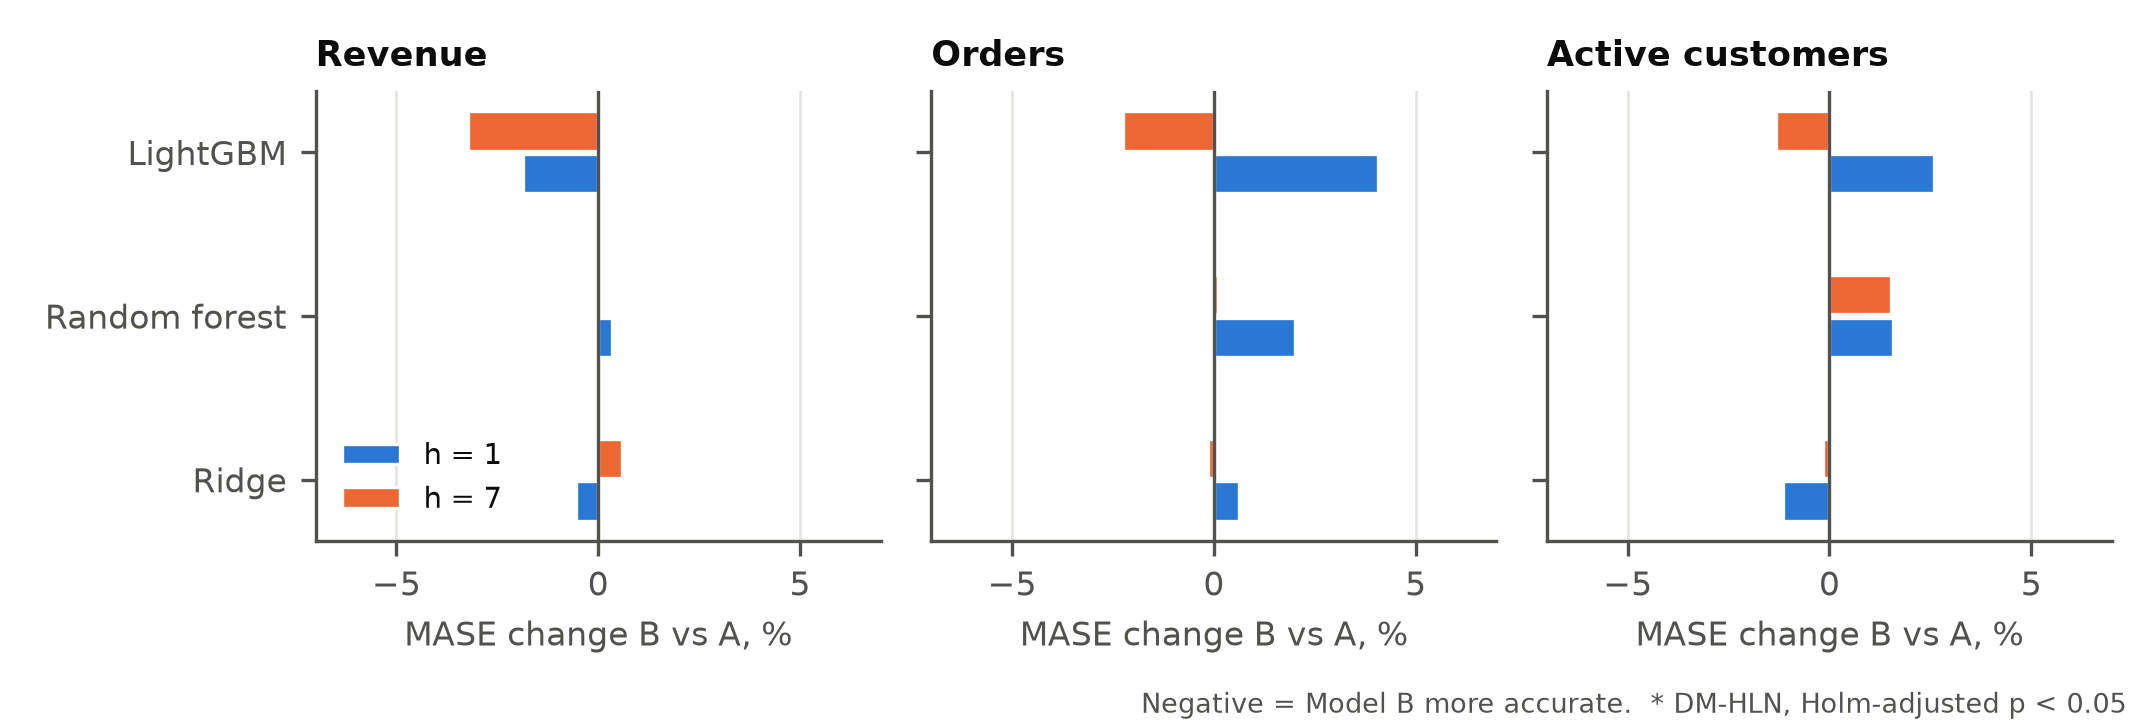
\includegraphics[width=\textwidth]{fig_rq2_b_vs_a_h17.png}
\caption{Relative MASE change of Model~B vs.\ Model~A for each target, model and horizon $h\in\{1,7\}$
(negative: Model~B more accurate). No difference is significant (Holm-adjusted DM-HLN, $p\ge0.05$).}
\label{fig:bva}
\end{figure*}

\subsection{RQ3: horizons and feature attributions}
Descriptively (Table~\ref{tab:mase}), from $h=1$ to $h=28$ the MASE of random forest (Model~A) rises from
0.752 to 0.758 and that of Ridge (Model~A) from 0.796 to 0.818, while LightGBM (Model~A) falls from 0.849 to % metrics.csv: mase_rev_random_forest_A_h1/h28, mase_rev_ridge_A_h1/h28, mase_rev_lightgbm_A_h1/h28
0.787; seasonal naive rises from 0.981 to 1.065, ETS from 0.872 to 0.920 and SARIMA from 0.838 to 0.960.
% metrics.csv: mase_rev_seasonal_naive_-_h1/h28, mase_rev_ets_-_h1/h28, mase_rev_sarima_-_h1/h28
Fig.~\ref{fig:shap} shows the share of mean absolute SHAP values by feature group for LightGBM with Model~B.
The lagged driver KPIs receive 48\%, 44\% and 41\% of the attribution at $h=1$, 7 and 28,
% shap_groups.csv: shap_drivers_B_h1/h7/h28_pct
although no statistically significant accuracy gain from them was detected at $h=1$ and $h=7$.
% dm_tests.csv: n_b_better_sig_h17_se, n_b_better_sig_h17_ae (0, 0)
The calendar share grows with the horizon (14\% to 27\% in Model~B; 26\% to 39\% in Model~A).
% shap_groups.csv: shap_calendar_B_h1/h28_pct, shap_calendar_A_h1/h28_pct
Group permutation importance ranks the calendar group first for both Ridge and LightGBM at all horizons. % permutation_importance.csv: perm_top_*

\begin{figure}[t]
\centering
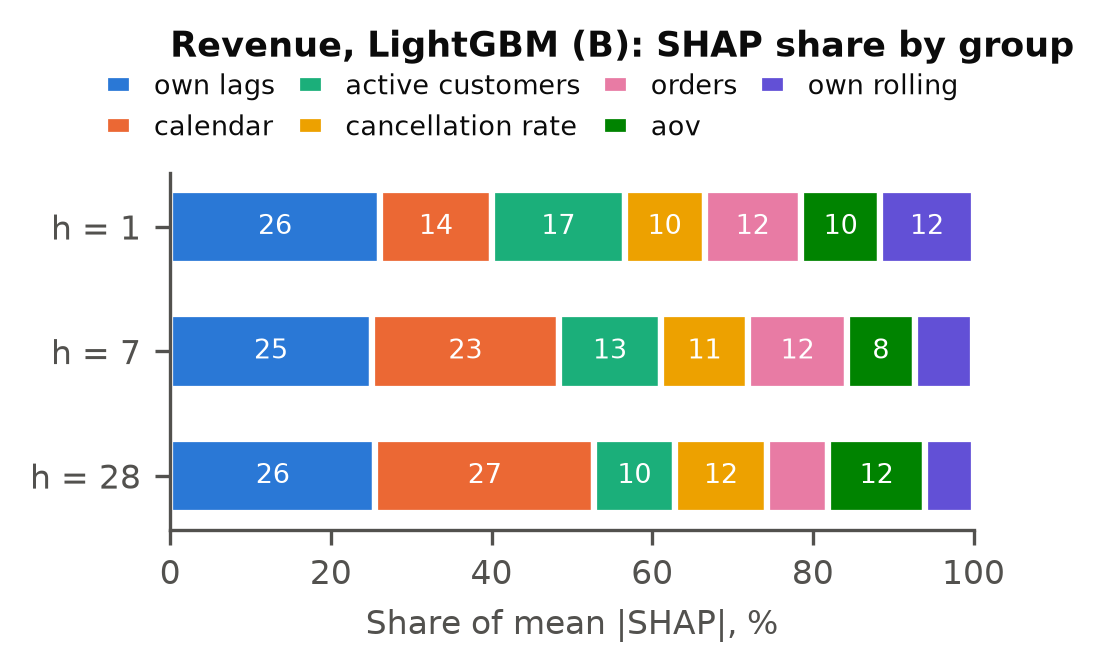
\includegraphics[width=\columnwidth]{fig_rq3_shap_groups.png}
\caption{Share of mean $|$SHAP$|$ by feature group for out-of-sample LightGBM revenue forecasts (Model~B).
Shares sum to 100\% before rounding; displayed values are rounded.}
\label{fig:shap}
\end{figure}

\subsection{Leakage control}
Adding the target day's own KPIs reduces the MASE of Ridge and LightGBM from 0.77--0.83 to 0.16--0.24 % leakage_control.csv: legal_mase_min/max, leak_mase_min/max
(Fig.~\ref{fig:leak}); the ratio of the legitimate to the leaky MASE is 3.4--4.8. % leakage_control.csv: leak_ratio_min/max (= MASE B / MASE leaky, per model and horizon)
For LightGBM at $h=1$, WAPE falls from 0.311 to 0.068. % leakage_control.csv: legal_wape_lgbm_h1, leak_wape_lgbm_h1
The added target-day features are unavailable at the forecast origin, so such forecasts cannot be issued.

\begin{figure}[t]
\centering
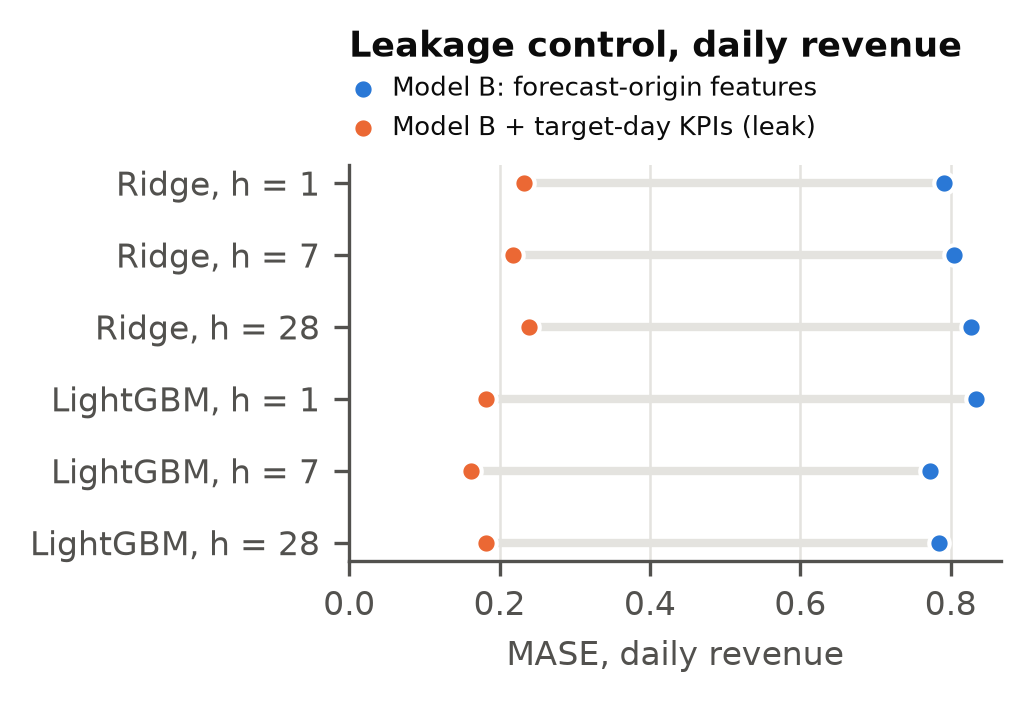
\includegraphics[width=\columnwidth]{fig_leakage_control.png}
\caption{MASE for daily revenue of Ridge and LightGBM with Model~B features available at the forecast origin
and with the target day's own orders, active customers, AOV, cancellation rate and quantity sold added
(leakage); all horizons, descriptive.}
\label{fig:leak}
\end{figure}

\subsection{Robustness}\label{sec:robust}
Excluding Saturdays, on which revenue is almost always zero, raises all MASE values (seasonal naive: 1.142 at % metrics.csv: mase_rev_nosat_sn_h1
$h=1$). Among Model~A configurations at $h=1$, Ridge (0.851) is slightly ahead of random forest (0.875), % metrics.csv: mase_rev_nosat_ridgeA_h1, mase_rev_nosat_rfA_h1
and the lowest MASE on this subset is Ridge with Model~B (0.844). % metrics.csv: mase_rev_nosat_ridgeB_h1
On this subset none of the 18 B-vs-A comparisons at $h=1$ and $h=7$ is significant under either loss; % dm_tests_no_saturdays.csv: n_b_vs_a_nosat_h17_se, n_b_sig_any_nosat_h17_se, n_b_sig_any_nosat_h17_ae
removing Saturdays leaves gaps in the forecast sequence, so the DM variance is an approximation here.

% =====================================================================================
\section{Discussion and Limitations}\label{sec:limits}
No statistically significant improvement from the lagged driver KPIs was detected in our setting, which is
consistent with the non-significant gain reported by~\cite{kim2026drivers} for a very different design. One
hypothesis is that at daily frequency the lagged drivers largely duplicate information already contained in
lagged revenue, so the models redistribute attribution (Fig.~\ref{fig:shap}) without gaining accuracy. We did
not test this hypothesis directly.

The leakage control shows why protocol details matter: with the target day's KPIs a model would reach a MASE
3.4--4.8 times lower than the legitimate models, and such a result could easily be reported as a success. % leakage_control.csv: leak_ratio_min/max

Limitations: (i) a single online retailer whose sales are mostly domestic (United Kingdom: 85.4\% of gross % eda_country_share.csv: uk_share_revenue_pct
revenue and 92.0\% of transaction lines), with one test year that includes one Q4 peak; % eda_country_share.csv: uk_share_lines_pct
(ii) Random forest and LightGBM used fixed hyperparameters; tuning inside each training window was not
attempted. LightGBM is weaker than random forest and Ridge at $h=1$ (MASE 0.849 vs.\ 0.752 and 0.796), so its
% metrics.csv: mase_rev_lightgbm_A_h1, mase_rev_random_forest_A_h1, mase_rev_ridge_A_h1
ranking should not be generalized; (iii) ML models are re-estimated weekly rather than daily; (iv) identical
transaction lines were treated as duplicates because the data contain no line numbers; (v) we did not
estimate the minimum detectable effect;
(vi) $p$-values for $h=28$ are computed and stored with the results but not interpreted: with 27 equally
weighted sample autocovariances and 305 forecasts, the protocol variance estimate is unstable. Among the 66
squared-error comparisons at this horizon (51 main comparisons for the three targets and 15 ablation % dm_variance_diagnostics.csv: dmvar_h28_n_tests, dmvar_h28_n_main, dmvar_h28_n_ablation
comparisons for revenue), it is positive but below half of the lag-0 variance in 7 cases and negative in 1; % dm_variance_diagnostics.csv: dmvar_h28_n_small_positive, dmvar_h28_n_negative_se
with absolute error it is negative in 2 further ablation comparisons.
% dm_fallback_counts.csv: fallback_h28_ae
Small positive variance estimates can inflate the magnitude of the test statistic; negative values trigger a
fallback to the lag-0 variance. No fallback occurred at $h=1$ or $h=7$;
% dm_fallback_counts.csv: fallback_h17_total
a corrected estimator is left for future work; (vii) the feature-group
ablation, the no-Saturday tests and the Bartlett check were added after the main results; (viii) deep
learning models were not considered.

% =====================================================================================
\section{Conclusion}
Under a leakage-safe rolling-origin protocol, ML models forecast daily revenue of an online retailer
significantly better than a seasonal naive baseline at 1 and 7 days under both squared and absolute error.
Against ETS, under absolute error 4 of 6 ML configurations are significantly better at 1 day and 6 of 6 at
7 days; under squared error only random forest with Model~A at 7 days is, and only with Bartlett weights.
Adding lagged
orders, active customers, AOV and cancellation rate together produced no statistically significant improvement
at 1 and 7 days for any model and any of the three targets; for revenue, the post hoc ablation that adds one
group at a time found no significant improvement either. Adding the target day's own KPIs, which are
unavailable at the forecast origin, would lower MASE by a factor of 3.4--4.8. At 28 days the ML models have lower
MASE than ETS and SARIMA, but the $p$-values at this horizon are not interpreted until a suitable variance
estimator is used. We recommend that KPI forecasting studies report leakage controls together with feature-group
ablations and significance tests whose variance estimator suits the horizon. Future work will replicate the
protocol on other retail data and at weekly frequency.

% =====================================================================================
\section*{Acknowledgments}
\CHECK[: thank supervisor M.\,Zh.\ Sergaziev and AITU if appropriate]

\bibliographystyle{IEEEtran}
\bibliography{references}

\end{document}
